%!TeX root=../tese.tex
%("dica" para o editor de texto: este arquivo é parte de um documento maior)
% para saber mais: https://tex.stackexchange.com/q/78101

\chapter{Arquitetura}

Neste capítulo, os pontos a respeito da organização e estruturação da
arquitetura que moldaram o formato do projeto, serão descritos com alguns
detalhes, primeiramente, destacando alguns tópicos adotados referentes ao
conceito de código limpo e por fim detalhando a modelagem do banco de dados e a
explicação da construção de suas entidades e relações.

\section{\textit{Clean Code}}

Um bom projeto não se resume apenas em eficiência na execução do programa ou em
um visual atraente para o usuário, outro ponto de grande importância, que
muitas vezes auxilia no alcance das qualidades citadas, é uma boa organização
de como os arquivos vão ser estruturados e separados por escopo.

Como descrito no capítulo 2 deste documento, houve uma separação base da
estrutura do projeto em três diferentes frentes. Além deste formato, durante o
desenvolvimento do trabalho, a arquitetura dos arquivos dentro destes tópicos
macro sempre foi um tópico recorrente, de forma que fosse possível manter uma
boa qualidade sobre o código que estava sendo escrito, ponto este, que foi
constantemente abordado durante toda a graduação ao longo de disciplinas como
MAC0218 (Técnicas de Programação II).

Assim como relatado por ~\citet{cleanCode} em \textit{Clean Code: A Handbook of
    Agile Software Craftsmanship}, um código pode ser considerado limpo se é
compreendido facilmente por desenvolvedores que não necessariamente
participaram do processo de desenvolvimento, o que torna muito mais viável uma
possível manutenção ou melhoria futura no código. Este ideal consiste de um
conjunto de conceitos básicos que em conjunto melhoram o entendimento do que é
escrito.

Nomes de variáveis e funções autoexplicativos, métodos enxutos e que possuam
uma responsabilidade única e bem definida, trechos de código relacionados entre
si próximos, consistência de códigos similares em lugares diferentes, aplicação
de padrões de projetos arquiteturais, testes unitários e uso de estruturas de
dados foram alguns dos diversos tópicos que foram utilizados no desenvolvimento
e que corroboram para a caracterização de um código limpo.

\begin{multicols}{2}
    \centering
    \vspace*{\fill}
    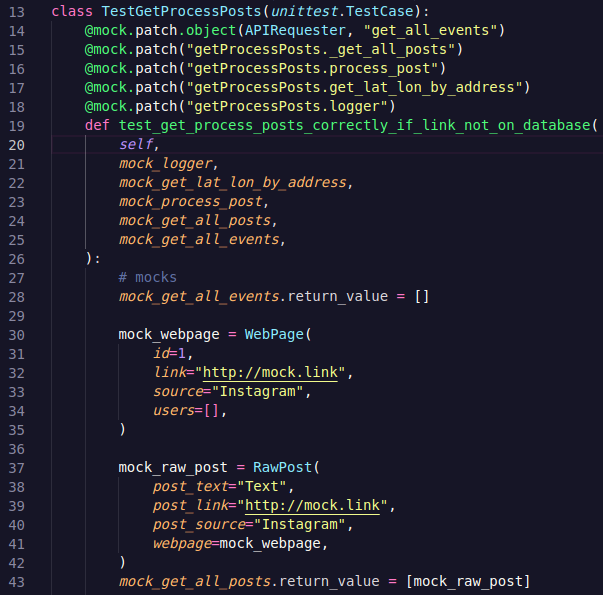
\includegraphics[width=0.4\textwidth]{figuras/testeUnitario1.png}
    \captionof{figure}{Exemplo de Teste unitário (1)}
    \vspace*{\fill}

    \vspace*{\fill}
    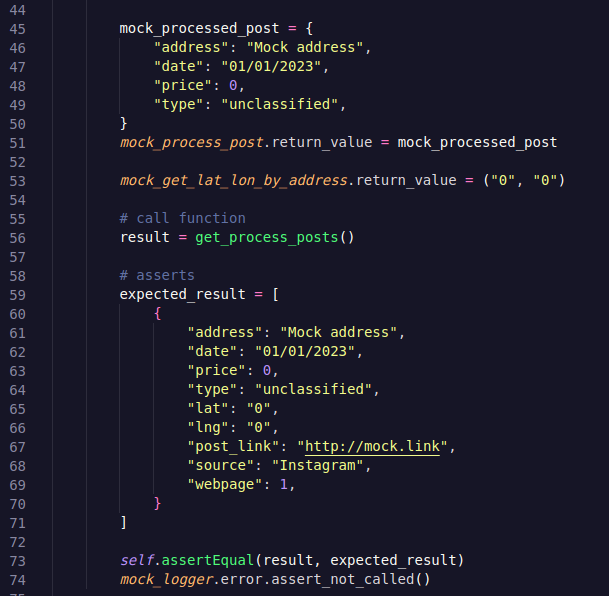
\includegraphics[width=0.4\textwidth]{figuras/testeUnitario2.png}
    \captionof{figure}{Exemplo de Teste unitário (2)}
    \vspace*{\fill}

    % \columnbreak

    % \vspace*{\fill}
    % 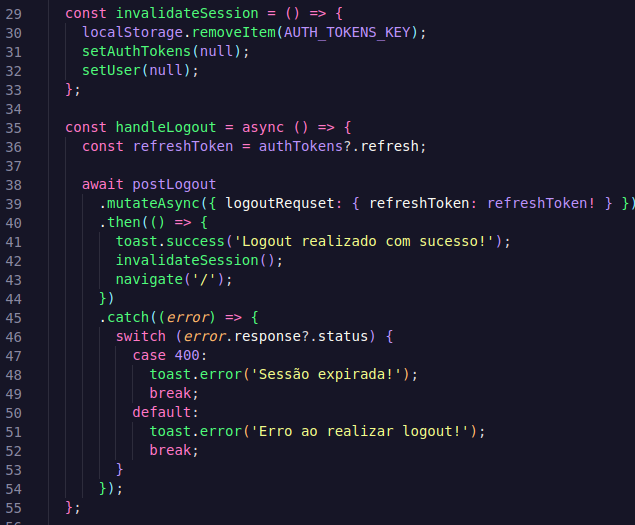
\includegraphics[width=.99\linewidth]{figuras/metodosRelacionados.png}
    % \captionof{figure}{Exemplo de métodos relacionados}
    % \vspace*{\fill}
\end{multicols}

\section{Banco de Dados}

O banco de dados foi modelado de uma maneira que pudesse se manter simples, mas
ao mesmo tempo fosse capaz de atender as necessidades para a estruturação do
projeto, para isso, algumas disciplinas cursadas durante a graduação como
MAC0350 (Introdução ao Desenvolvimento de Sistemas de Software) e MAC0426
(Sistemas de Bancos de Dados) contribuíram com os conceitos básicos utilizados.

\begin{figure}[h]
    \centering
    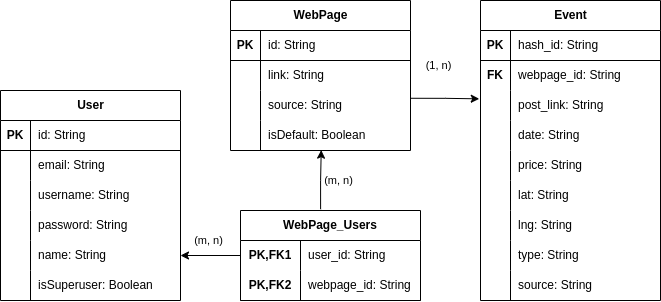
\includegraphics[width=1\textwidth]{figuras/typesTCCModel.png}
    \caption{Modelo do banco de dados utilizado}
    \label{fig:enter-label}
\end{figure}

Existem três principais entidades definidas no modelo. Para cada uma, existem
\acp{API} responsáveis pela criação, deleção ou edição delas. Algumas destas
\acp{API} necessitam de privilégios de administradores para serem utilizadas. A
seguir estão alguns detalhes com respeito às entidades e tabelas modeladas:

\subsection{\textit{User}}

A tabela de \textit{User} armazena informações a respeito dos usuários da
plataforma. Um novo usuário é criado toda vez que a ação de cadastro é feita
dento da plataforma a partir de informações básicas como nome de usuário, senha
e \textit{email} por exemplo. O armazenamento da senha criada no registro é
armazenada de forma criptografada dentro do banco para garantir uma maior
segurança dessa informação.

Existem dois tipos de usuários, os criados através do fluxo descrito são
usuários padrões, enquanto que usuários criados utilizando a \acs{API}
direcionada à uso exclusivo de administradores são chamados de \textbf{super
    usuários}. Os tipos de usuários podem ser diferenciados no banco de dados
através do campo \textit{isSuperuser} da tabela \textit{User}.

\subsection{\textit{WebPage}}

A tabela \textit{WebPage} é utilizada para guardar informações relacionadas às
páginas de redes sociais de preferência cadastradas pelos usuários dentro da
plataforma. O sistema utiliza destas \textit{webpages} cadastradas para buscar
as informações necessárias para criação do evento que será exibido dentro da
plataforma futuramente.

Como descrito no parágrafo anterior, as \textit{webpages} são o ponto inicial
para que um evento seja gerado, porém, existem situações em que um usuário
deseja utilizar a plataforma sem a necessidade de realizar um cadastro,
consequentemente, não haverá nenhuma \textit{webpage} de preferência criada por
ele. Dessa forma, inicialmente o sistema possui \textit{webpages} padrões de
onde serão extraídos os eventos mostrados para todos os usuários, com e sem
cadastro na plataforma.

É importante ressaltar que atualmente o sistema dá suporte para páginas que sejam do \textit{Facebook} ou do \textit{Instagram}, por isso, a própria plataforma restringe a criação das \textit{webpages} de uma destas duas fontes, representado pelo campo \textit{source} na tabela.

\subsection{Event}

A tabela \textit{Event} é responsável pelo armazenamento dos eventos gerados a
partir das \textit{webpages}. Os textos que são obtidos dos \textit{posts}
publicados nessas páginas passam por uma etapa de processamento onde são
extraídas as informações necessárias para a construção dos eventos. Dessa
forma, é estabelecida uma relação entre as entidades \textit{Event} e
\textit{Webpage} onde uma \textit{webpage} pode possuir um ou mais eventos
diferentes.

A princípio, a partir do processamento os eventos são diferenciados em dois
tipos que são esportivos (\textit{sport}) ou cultura (\textit{culture}),
entretanto, existem casos que o modelo não consegue classificar corretamente o
evento em um desses tipos, assim, estes são mantidos como não classificados
(\textit{unclassified}). Os diferentes tipos de eventos são identificados
dentro do sistema através do campo \textit{type} na tabela \textit{Event}. Essa
entidade ainda possui um campo de \textit{id} que utiliza um sistema de
\textit{hash} que utiliza o \textit{link} do post com os dados do evento para a
geração desse \textit{id}.

\subsection{WebPageUsers}
\label{sec:WebPageUsers}

Essa tabela foi criada para funcionar como um intermediário entre as entidades
de \textit{Event} e \textit{WebPage}. Essa relação tem o intuito de tornar
possível atrelar um usuário aos eventos obtidos através de uma \textit{webpage}
cadastrado pelo usuário. Além disso, como a relação entre estas entidades
mencionadas foi estabelecida, também é possível criar uma relação para
identificar quais usuários realizaram o cadastro de cad uma das
\textit{webpage} existentes.
